\section{Outlier Detection based on representation learning}


This section will be about the newly proposed Intercont method of \citep{shenkar2022anomaly}. 
Leading to that and to give background knowledge, the basics of machine learning will be described.
I begin with traditional machine learning paradigms and define the paradigm which is used in the InterCont method.
I will discuss pros and cons of each paradigm.


%\begin{figure}[H] 
%    \centering
%    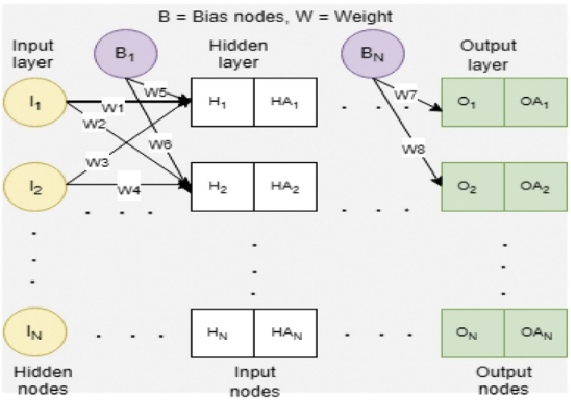
\includegraphics[trim={-100pt -100pt -100pt -300pt}, clip, width=\textwidth]{Images/Neural_network_architecure}
%    \vspace{-100pt}
%    \caption{Architecture of the Neural Network}
%    \label{fig:nn_arch}
%\end{figure}
\todo{reject image?}


Rather than focusing on isolated methods, machine learning paradigms function as overarching frameworks for interpreting data. 
While specific algorithms act as individual components, the paradigm itself offers the "big picture" view necessary to navigate the field.
Therefor most methods can be implemented in different paradigms.
Generally there are three traditional machine learning paradigms:
Supervised, unsupervised, reinforcement learning.   
There are plenty of different subtypes of learning paradigms. 
For further information I recommend the survey of \citet{sarker2021machine}.
In the paper the authors depict not well known paradigms like semi-supervised learning, multi-label learning or transfer learning.


The most widley used paradigm is the supervised learning. 
Supervised learning is mostly used for classification and regression tasks.
In supervised learning, the model ist tranined on labled data. 
The label defines the correct anwer for the model in advance.
The models goal is to learn a mapping function.
Depending on the task, the model is capable to presenting a satisfiying answer, if its presented new unseen data.
Therefor it is also named an task-driven approach. \citep[p.3]{sarker2021machine}
On the one hand, supervised learning leads to results with high accurarcy, reliable predictions and its performance is easy to measure.
On the other hand, it requires labled data, wich are highly cost and time intensive to generate.
Furthermore it could struggle with new unseen scenarios that are not in the training data.


In unsupervised learning, the training data is unlabled. 
Its an data-driven approach.
It is only provided input data but no corresonding output lables or supervision.
The goal is to explore the data, find hidden patterns, and discover the underlying structure or distribution within the data on its own.
Its about drawing inferences rather than making predictions with predefined answers.
For unsupervised learning there is no need for costly curated datasets, and the models can handle large data volumes.
It is perfect for finding hidden patterns, structures groupings and relationsships in the data.
But the models are not as accurate as supervised counterparts and its interpretability is more complex because there is no objective trith to measure against.
The models tend to be computational intensive espacially with large datasets. The results tend to be noisy.
\cite[p.4]{sarker2021machine}


The method of \citet{shenkar2022anomaly} uses a self-supervised learning which is often credited as a type of unsupervised learning.
It's goal is to label the data on its own and therefor does not need human intervention mitigating the problem of costly data labeling.
Nevertheless it has supervised characteristics as well.
It uses loss functions to measure its performance against labels wich it self created.
In cases, e.g. Computer Vision, where a potentially a high number of classes can emerge, it is more suitable to design a model wich can fulfill this task alone. 
Introducing metric learning, where the goal is to generate a numerical representation of the input, as a image, and putting it into an embedding space resulting in a vector.
This initial vector is called anchor. New images are added and the network learns an embedding space, where simmiliar images are put cloder together and dissimiliar 
images are put further away. When the network is presented with a slightly different version of the anchor image, the network is capable of recognizing the most important 
aspects of this image, because it puts the new image near the anchor in the embedding space.  
Those networks reduce complexity by reducing the dimensionality of the input.
If a new datapoint is introduced, the model embedds the data and and classifies the data accourdingly to the localtion in the embedding space. 
\citep{raina2007self}
\todo{the difference between unsupervised and self-supervised learning?} 


\subsection{Neural Network}
In this section I will describe the traditional architecture of a neural network (NN)
I will concentrate on the main building blocks: Layers, activation functions and loss functions. 
A neural network is a model inspired by the structure and function of the human brain. 
It is suitable for a lot of tasks: for example classification, clustering, pattern recognition and predictive tasks.
The goal is to construct a generalizable model.
That means, that the model performs on unseen data nearly as good as on the training data \todo{check statement}
\todo{insert example papers maybe in the financial domain?}


The arcitecture of a neural network consists of layers. 
Those layers consist of nodes, wich are mathematical functions.
The first layer is the input layer and it receives the raw data. 
Each node in the input layer corrensponds to a feature in the data.\todo{is that right?}
After performing the first computation through the node, the result is pushed to the next layer, called hidden layer.
The network can be made up of aribrary number of hidden layers. 
Models that use one hidden layer are called shallow network and models that use more than two hidden layers are referred to as "deep networks".
The more hidden layers are used, the more complex pattern recognition can be done by the network.
With deep learning, high dimensional data can be processed effectively.
Between layers there are the weights, biases and activation functions. 
The weight determines how important the connection between these two nodes are. 
The more imporant it is, the higher the weight. 
The bias is a value that determines if the node should pass the result to the next layer. \todo{is that right?}
If the threshold is met, the node is passing the result to the next layer.
Until the last layer, called  output layer, is reached.
The output is compared to the real value of labled data using a loss function. 
After calculating the loss, the model uses backpropagation to send the result backwards thought the layers.  
By using the chain rule, the model calculates how much each weight and bias contributes to the loss, called gradient.
An optimizer is been used to adjust the bias and weights. 
The goal is to minimize the loss function and getting an generalizable model that can be applied to new unseen data.
By restarting this cycle an epoch is fulfilled. 

\todo{consider: example of chain rule?}
\todo{explain why backpropagation needs differentialablity}


An activation function is influences the models ability to approximate the target function.
The approximation of a network using just linear activation functions have to be linear too.
To introduce non-linearity into the model an activation function is used. 
The model passes the input by multiplying the input (X) with the initial weight (W) and adds a bias (b). 
The activation function (omega) assigns a value to the incoming input.
The activation functions have to be non-linear, differential and monotone increasing. 
In the next step, the value is passed the output onto the next layer.


\subsubsection*{Activation Function}
The most commonly used activation functions are logistic/sigmoid, tanh and ReLU.
For further information about less known activation functions, I recommend the survey of \citep{nwankpa2018activation}. 
\todo{find credable journal}
The logistic function is defined as: 


\begin{equation}
    z = \frac{1}{1 + e^{-x}}
\end{equation}


%\begin{figure}[t] 
%    \centering
%    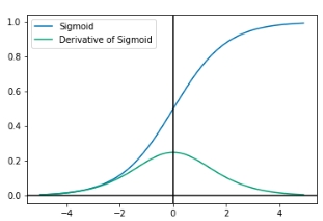
\includegraphics[trim={-100pt -100pt -100pt -300pt}, clip, width=\textwidth]{Images/Sigmoid.pdf}
%    \caption{Architecture of the Neural Network}
%    \label{fig:nn_arch}
%\end{figure}


A logistic function is bounded to an intervall of 0 to 1, therefore the model can interpret it as probabilities.
The "S-shaped" function meets the above presented requirements.
The maximum is derivated at z=0 is 0.25.
This allows for a smooth gradient preventing jumps in output values resulting in more stable results.
A mayor issue is the vanishing gradient problem.
For extrem input values, the function produces satured/ flat outcomes. 
If the model backpropagates,the small gradients are multiplied and therefor shrinking until its nearly zero and the model stops learning.
In addition the output is not zero-centered. The results are lay between zero and one. 
This causes the gradient to be all negative or all positive, resulting in a undesirable dynamics.
Because an exponential function is used, the computational costs are high compared to other modern activation functions


The hyperbolic tangent (tanh) activation function is used to resolve some of the criticism of logistic function. 
It is defined as: 

\begin{equation}
    \tanh(z) = \frac{e^{x} - e^{-x}}{e^{x} + e^{-x}}
\end{equation}


%\begin{figure}[H] 
%    \centering
%    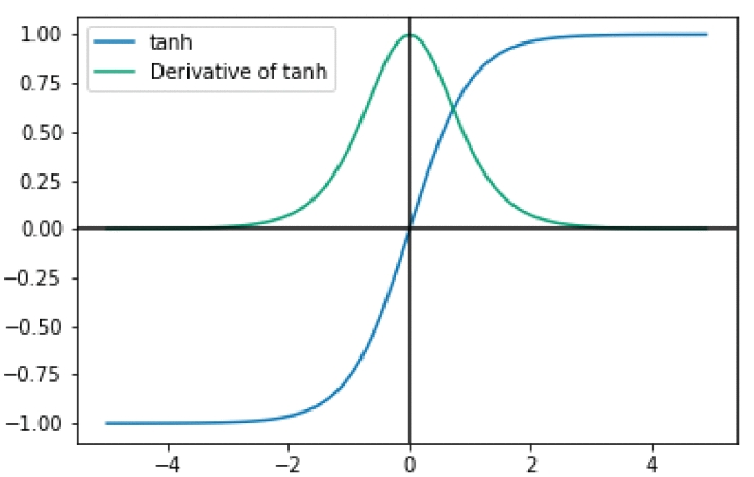
\includegraphics[trim={-100pt -100pt -100pt -300pt}, clip, width=\textwidth]{Images/Tanh.pdf}
%    \vspace{-100pt}
%    \caption{Architecture of the Neural Network}
%    \label{fig:nn_arch}
%\end{figure}


Its is a scaled and shifted version of the logistic function centered around zero.
Therefore the values lay between -1 and 1. 
The output mean is more centered around zweo resulting in a more balanced weights and faster convergence during training.
The maximum derivative is 1.0, resulting in a faster learning if the inputs are near zero.
The tanh activation function is not fully capable of solving the vanishing gradient problem.
On the one hand, the range of possible outputs is larger, therefor a gradient vanishes more rarer.
On the other hand, does the gradient still vanishes but with more extreme values than before.


The rectified linear unit (ReLu) activation funcion is used to eliminate the vanishing gradient problem completly.
The ReLu activation function belongs to the class of piecewise activation functions.
The ReLu is defined as: 

\begin{equation}
    f(z) = \max(0, x)
\end{equation}

%\begin{figure}[H] 
%    \centering
%    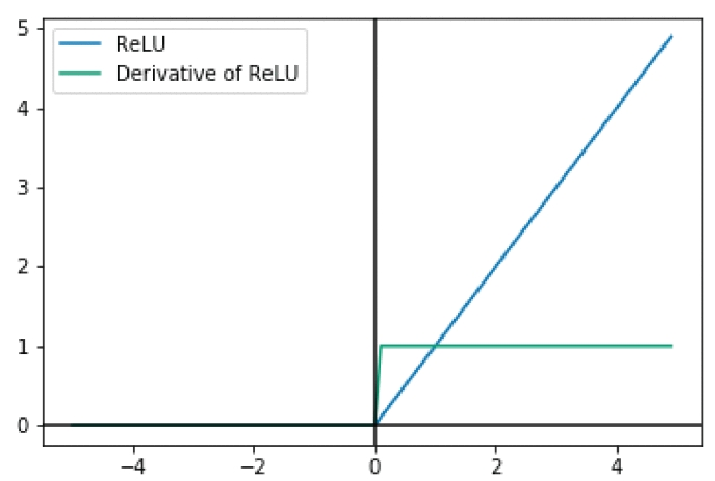
\includegraphics[trim={-100pt -100pt -100pt -300pt}, clip, width=\textwidth]{Images/ReLu.pdf}
%    \vspace{-100pt}
%    \caption{Architecture of the Neural Network}
%    \label{fig:nn_arch}
%\end{figure}

%\begin{figure}[H] 
%    \centering
%    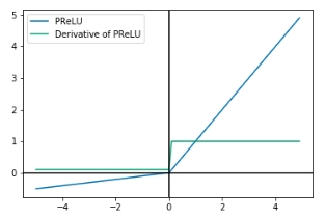
\includegraphics[trim={-100pt -100pt -100pt -300pt}, clip, width=\textwidth]{Images/Leaky_ReLu.pdf}
%    \vspace{-100pt}
%    \caption{Architecture of the Neural Network}
%    \label{fig:nn_arch}
%\end{figure}


The activation function produces a value of zero, if the input value is less than or equal to zero.
If the input is greater than zero, the ReLu function passes the input onto the output.
For all positive value the gradient is 1, solving the vanishing gradient problem even if the network consists of multiple hidden layers.
Nodes that receive a negative input, the activation function  assigns a value of zero, shutting the node off.
That leads to more efficient and lighter models but creating a problem, by making the node permantly inactive and not contributing to the network.
The Leaky ReLu activation function is solving this problem, by letting negative values backpropagate by a smaller factor.
The authors of the InterCont method used a LeakyReLU activation function to mitigate disadvantages of other activation functions.


\subsubsection*{Loss Function}
The loss function is a tool to measure the performance in the training procedure and leads the optimization of the bias and the wheights.
It depends on the networks architecture, the nature of the data and the task which loss function is suitable.
Traditional loss functions are the Mean squared error (MSE), Mean absolute error (MAE) and Huber loss. 
The loss is used for the optimizer, to determine the 
The authors of the InterCont methos used a special loss function, because they chose a contrastive learning architecture.
In the next chapter I will explain in more detail, how the contrastive loss function works.
For Further information and detail analysis of other loss functions, I recommend the survey of \citep{terven2025comprehensive}


\subsubsection*{Optimizer}
An optimzer is used to determine the biases and wheights in a NN. 
When the network backpropagates, the initial biases and wheigts have to change, to minimize the loss function. 
Most optimizers are based on Gradient descent.
The gradient is calculated by deriving the loss with respect to each weight.
The goal is to find the direction of the gradient.
The optimizer shift the weights in taht downhill direction.
Using the learning rate, the optimizer is constraint in its step size. 
The smaller it is, the more epochs it need to minimize the loss function.
\todo{why do we use it}
\todo{describe Adam Optimzer}
\todo{find a good survey about optimizer}


\subsubsection*{Over and Underfitting}
Two common issues that affect a model's performance and generalization ability are overfitting and underfitting. 
These problems are major contributors to poor performance in machine learning models.


%\begin{figure}[H] 
%    \centering
%    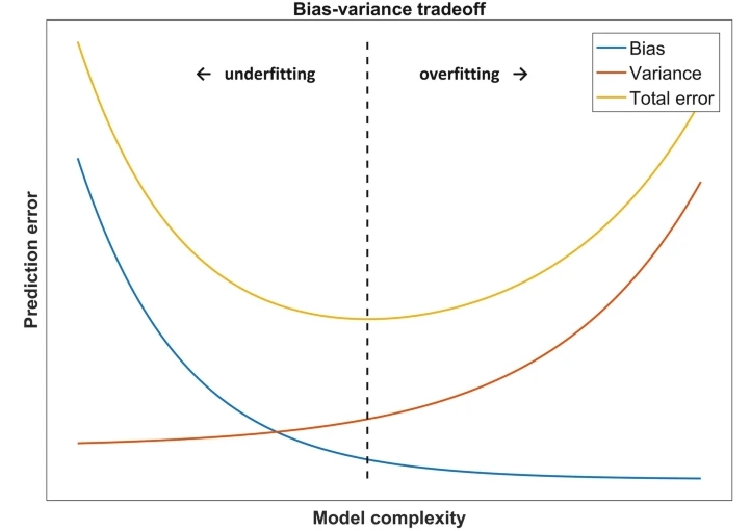
\includegraphics[trim={-100pt -100pt -100pt -300pt}, clip, width=\textwidth]{Images/Bias_Variance_Tradeoff.pdf}
%    \vspace{-100pt}
%    \caption{Architecture of the Neural Network}
%    \label{fig:nn_arch}
%\end{figure}


As depicted in the figure: Bias and Variance share a tradeoff relationship. 
Bias represents the error introduced by approximating a complex real-world relationship with a simplified model. 
High bias occurs when a model lacks sufficient complexity to capture the underlying patterns of the data, resulting in underfitting where performance is poor on both training and testing sets. 
Conversely, variance refers to the model's sensitivity to small fluctuations in the training set. 
High variance occurs when a model is overly complex, leading it to capture stochastic noise and outliers rather than the generalizable signal.
This state, known as overfitting, is characterized by high accuracy on training data but a failure to generalize to unseen datasets. 
To mitigate underfitting and reduce bias, one must increase model complexity, perform feature engineering to add relevant input variables, or extend the training duration to allow for better convergence. 
To address overfitting and reduce variance, techniques such as k-fold validation or batch are employed to penalize excessive model complexity. 
Additionally, increasing the volume of training data, implementing dropout layers in neural networks, or utilizing early stopping based on validation loss can prevent the model from learning noise. 
The objective of model selection is to minimize the sum of bias and variance to achieve optimal predictive performance.
\todo{k-fold validation for knn}
\todo{Batch trainig for Intercont}

\subsection{Contrastive Learning}
The proposed method of \citet{shenkar2022anomaly} applies an internal contrastive learning algorithm (InterCont) onto tabular data, which is an unseen application of contrastive learning, 
because that type of learning has seen significant attention in computer vision and natural language processing.
The goal is to build a network, that can destinguish between different instances, e.g. an image of a cat, and images of different animals. \todo{expression}
Therefore the netwroks needs to extract usefull information to discrimminate.
This chapter will define a framework to analyse contrastive learning algorithms. 
Therefore I will explain the main components. 
There are different ways of building an contrastive learning network, but main architecture converged into a stable structure. (Hu,p.6)
The chapter is organized as follows: First I will explain the data augmentation using data augmentation in computer vision as an example.
Then I will explain the traditional network structure.
That includes the encoder network, the projection head and sometimes the prediction head.
Lastly I will explain the main contrastive loss functions.
%%\input{Images/InterCont/Survey_Contrastive_Learning.pdf}


\subsubsection*{Data Augmentation}
The model is given an anchor, which is a specific piece of data (like an image) which represents the desired target to destinguish from. 
The model is given a positive sample by applying a random data augmentation technique.
For example in computer vision the most used data augmentation techniques include: cropping, flipping and rotating. 
Because this positive pair originated from the same source, the model placees them close together in the feature space.
There are different techniques for data augmentation.
For more information about data augmentation techniques in contrsative learning, I recommend \todo{insert survey about}


In contrast, a negative pair is formed by finding a different piece of data, hence the negative sample. 
The goal is to push the negative samples further away from the anchor as the positive samples.
The selection of negatives samples is a challenging task.
Negative samples have to be informative and challenging for the network, introducing diversity into the model.
Hard negatives are close to and semantically similiar to the anchor.\todo{insert paper Jang et al.}  
By training with many of these negative samples, the model becomes much better at identifying the unique details that set different objects apart.
This process prevents the model from overfitting the training data and mitigates problems concerning data biases, increasing the overall modells generalization performance.
But including an abitrary number of random data instances is not providing the needed hard negatives. 
It is always recommended to include the specific nature of the task and dataset, when curating negative samples to minize misleading influences. \todo{why?}
\todo{add: Methods of sampling negatives} 
\todo{add: Sliding window other papers that use that}
\todo{add: Sliding Window: critizms: geometric Concentration, syntax vs semantics trade off, selection bias and false negatives}


\todo{insert solution for sample selection to critize InterCont}


\subsubsection*{Network Structure}


%\begin{figure}[H] 
%    \centering
%    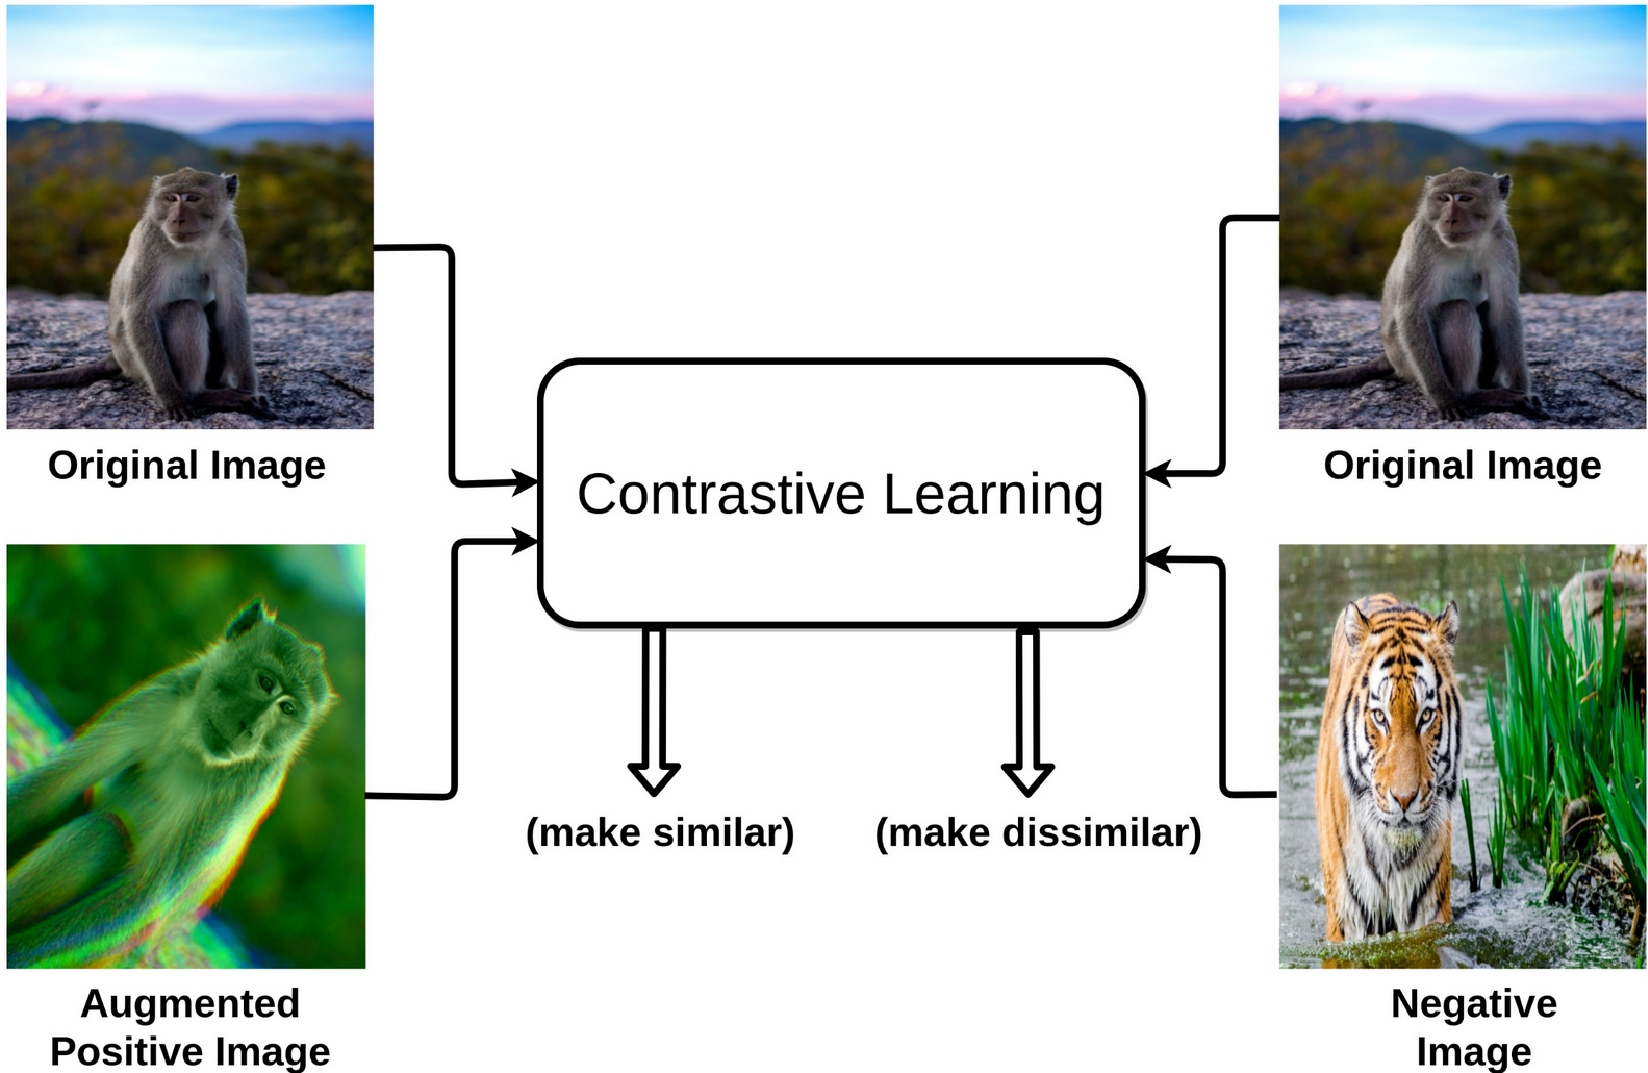
\includegraphics[trim={-100pt -100pt -100pt -300pt}, clip, width=\textwidth]{Images/Contrastive_learning_intuition.pdf}
%    \vspace{-100pt}
%    \caption{Architecture of the Neural Network}
%    \label{fig:nn_arch}
%\end{figure}


The encoder network takes the augmented instances as input and embedds them to the latent space, where meaningful features and similarities are captured. 
A latent space is a abstract, compressed and low-dimensional vector space of the input data, where essential features and underlying patterns are encoded.
The goal is to filter out noise and redundant information.  
The networks hidden layers 
They consists of two main parts: The encoder takes the high dimensional input and maps it to a much smaller vector in the latent space. 
This enforces the necessary compression.
The hidden layer is designed as a bottleneck, wich means it contain fewer nodes than the corresponding layer before. 
The decoder takes the compressed vector and attemps to reconstruct the original high dimensional input. 
The encoder is trained to minimize the difference between the original input and the reconstructed output. 
By forcing the information through the bottleneck, the enoder learns only the most essential features required for accurate reconstruction.
The output of the encoder network is pushed to the projection head.
\todo{insert momentum ecoder?}
That is a non-linear layer to refine the learned representations further. 
it is standard practice in most contrastive learning algorithms.
Some, like BYOL \todo{insert paper} do add another non linear layer, called prediction layer, to further enhance the results of the algorithm.


%\begin{figure}[H] 
%    \centering
%    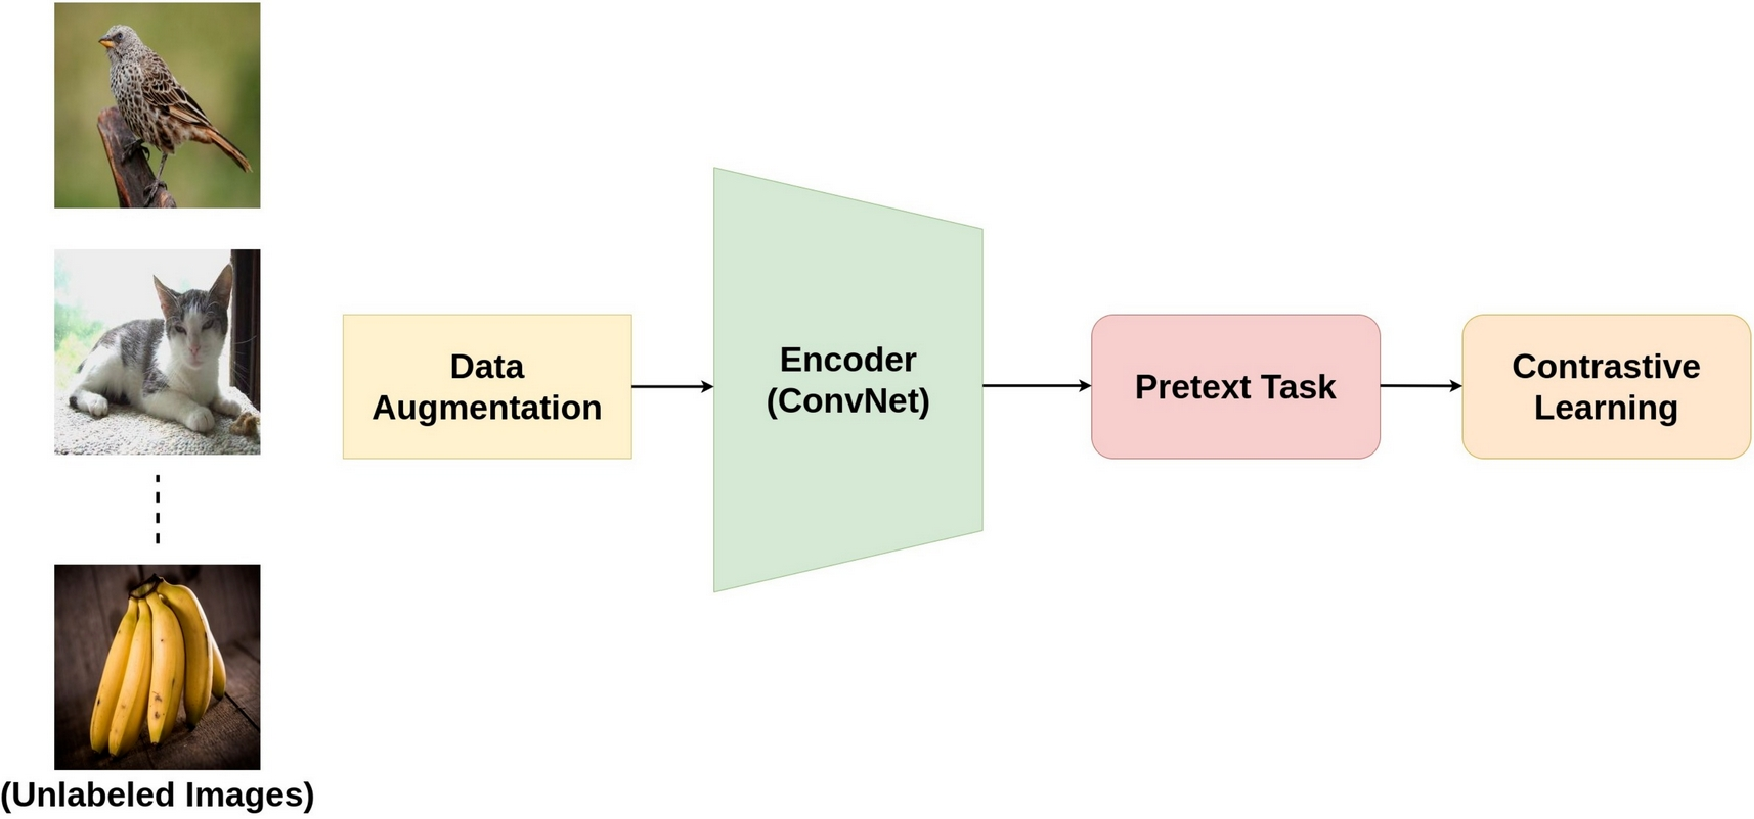
\includegraphics[trim={-100pt -100pt -100pt -300pt}, clip, width=\textwidth]{Images/contrastive_learning_pipeline.pdf}
%    \vspace{-100pt}
%    \caption{Architecture of the Neural Network}
%    \label{fig:nn_arch}
%\end{figure}


\begin{figure*}[htbp]
    \centering
    \begin{subfigure}[b]{0.498\textwidth}
        \centering
        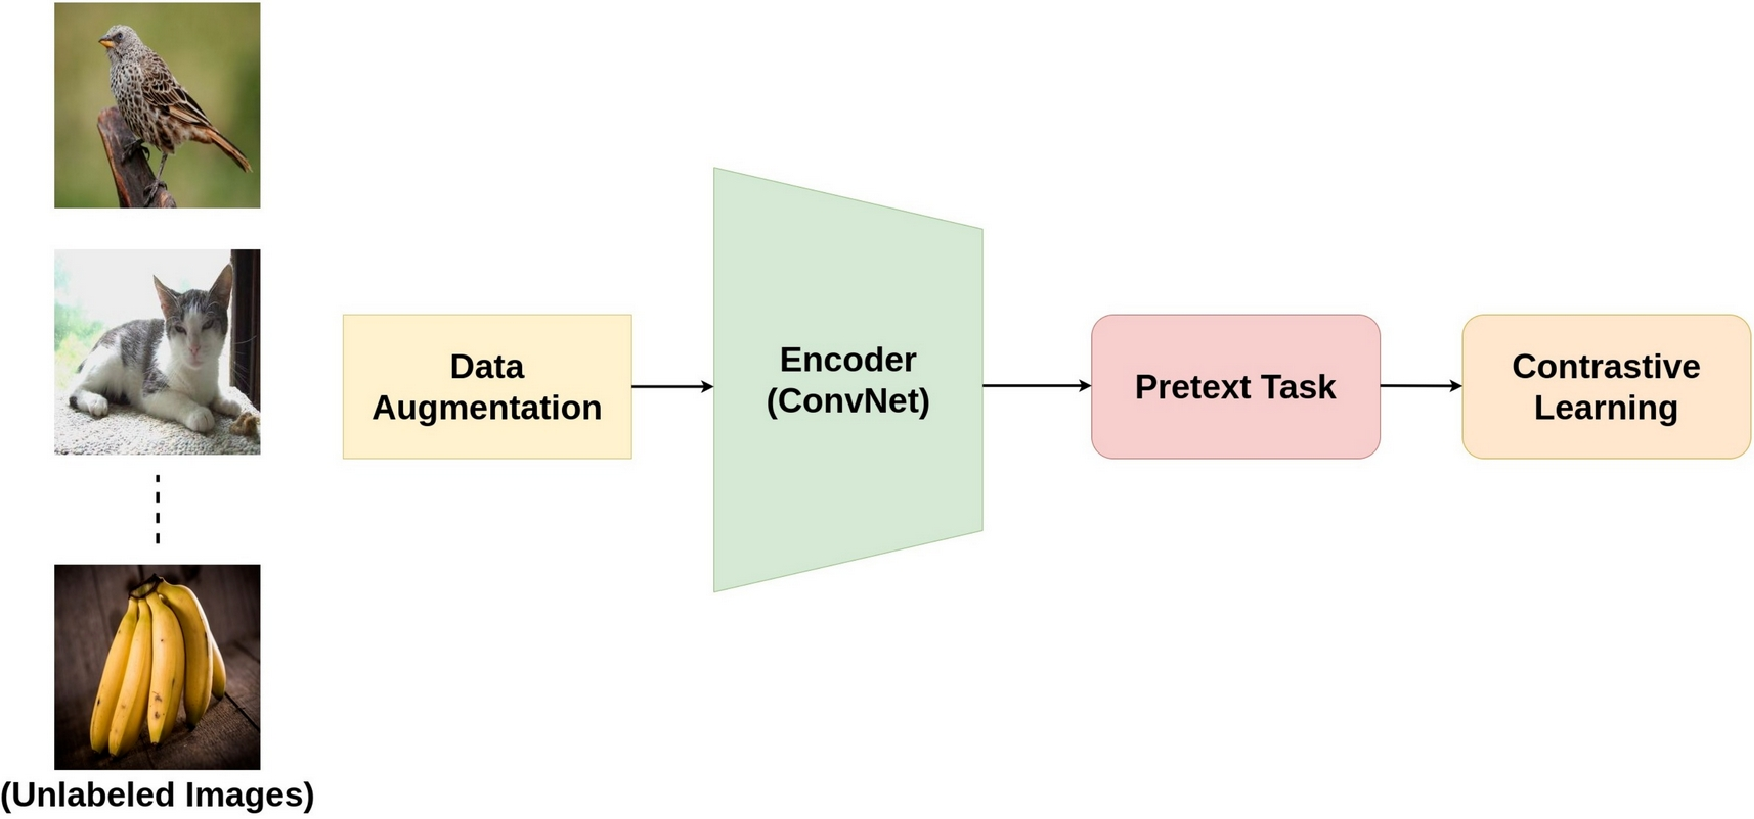
\includegraphics[width=\textwidth]{Images/contrastive_learning_pipeline.pdf}
        % \caption{Caption.}
        \label{fig:calvo_mse}
    \end{subfigure}
      \begin{subfigure}[b]{0.498\textwidth}
        \centering
        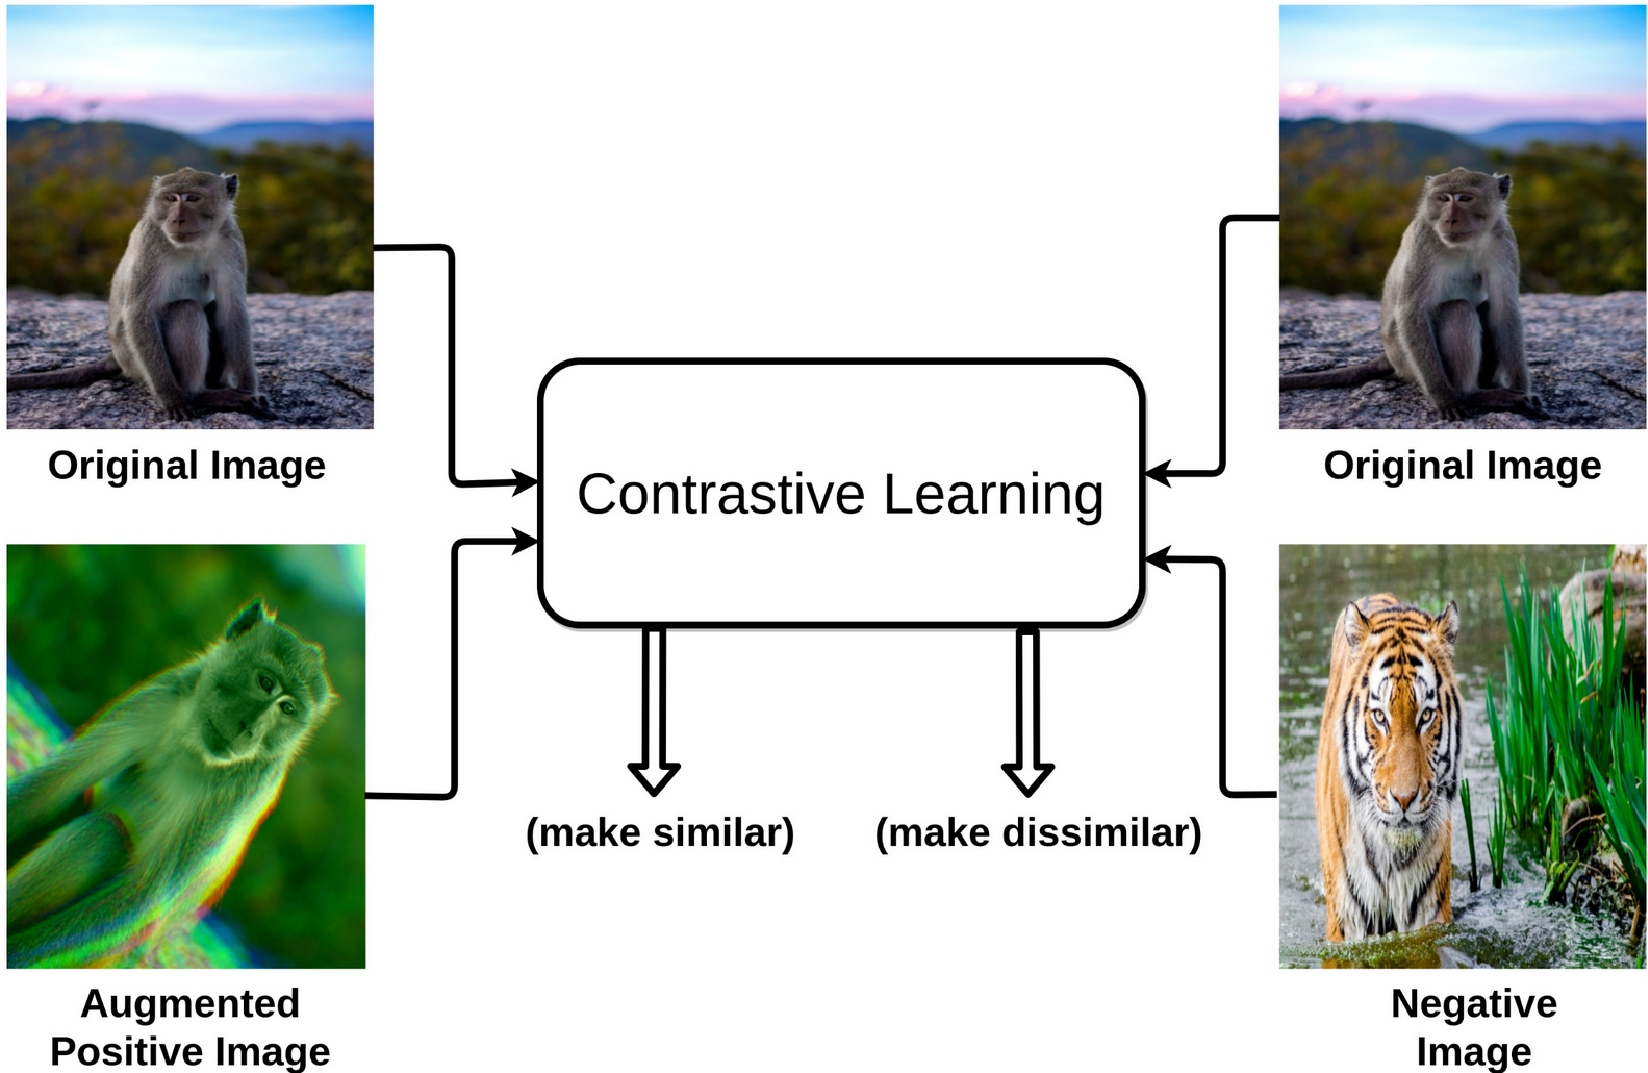
\includegraphics[width=\textwidth]{Images/Contrastive_learning_intuition.pdf}
        % \caption{Caption.}
        \label{fig:calvo_complexity}
    \end{subfigure}
    \caption{}
    \label{fig:calvo}
\end{figure*}

\subsubsection*{Contrastive loss function}
The contrastive loss function has a different goal, as the loss functions discussed in chapter 2.
The goal is to discriminate and minimze the distance between positive samples and the anchor and maximize the distance between negative samples and the anchor.
The specific choice of the loss function depends on the network arcitecture and the characteristics of the dataset. 
The most commonly used contrastive loss function  is the Info noise contrastive estimation (InfoNCE).
Nevertheless often in practice adjusted versions are implemented too.
To get an overview of different contastive loss functions I reccomend the paper of \todo{insert paper}
In this thesis I will concentrate on the InfoNCE, because thats the contrastive loss function used in the method of \citet{shenkar2022anomaly}.


\subsubsection*{Info noise-contrastive estimation (InfoNCE)}
InfoNCE is an optimized version of the noise contrastive estimation (NCE) proposed by \citet{gutmann2010noise}.
First published by \citet{oord2018representation}, the authors proposed an function that incorporates mutual information. 
InfoNCE maximized the mutual information between positiv pairs and minimized mutual information between negative pairs.
It is defines as: 


\begin{equation}
    \mathcal{L}_{N} = -\mathbb{E}_{X} \left[ \log \frac{f_k(x_{t+k}, c_t)}{\sum_{x_j \in X} f_k(x_j, c_t)} \right] .
\end{equation}


where xt+k represents the positive samples, xj represents the negative samples, fk represents the density ratio, so well the pairs match and N is the difficulty, a scaling facor for information.
This equation calculates an average of all the data and uses the log to deal with the exponential growth of the scores. 
The goal is to maximize the the probability of pciking the right sample. 
By adding a negatve sign to the los expectation, the equation minimizes the value. 
So if the probablity is 1 the loss will be 0.


The loss function maximizes the mutual information.
Mutual information refers to the information relationship between variables. 
It is a parameter that determines the knowledge of variables, depending on the knowledge of another variable. 
By minimizing the loss it is mathematically quaranteed, that the information shared between the data and the representation is maximized.
That means that the learn representation contains as much information of the data as possible resulting in the essence of the data.
For further mathematical proof, I recommend the paper of \citet{oord2018representation}
It also shows that the information is restricted by the number of negative samples. 
The more negative samples I add, the more information the method


\subsubsection*{Cross entropy loss}
Cross entropy loss measures the difference between a variables predicted distribution and it actual distribution.
It's often used for classification problems.
In contrastive learning, the training set is ofter divided into batches.
and it's defined as follows: 
\todo{add:why do we used batches here?}
\todo{research: cross-entropy and the loss function in Wu 2018, He 2020}


\subsection{InterCont}
This chapter will be about the proposed internal conrastive learning algorithm of \citeauthor{shenkar2022anomaly}.
The goal is to determine a score y, that assigns a low value for samples that are samples from the underlying distribution.
Otherwise the score should by higher.
I will begin by explaining the main hyperparameters and initialization of the model.
To exert the framwork discussed above, I will compare and explain the data augmentation techniques of InterCont with the framwork ones.
Followed by a description of the networks structure and ending with the chosen contrastive loss function.


The model has two main hyperparameters: 
\begin{enumerate}
    \item k determines the number of consecutive number of the features to form the positive sample a (hereby k < d).
    \item u determines the embedding size.
    \item Tau is a temperature constant in the contrastive loss function.
\end{enumerate}


The authors proposed a sliding window approach for data augmentation. 
The model initializes by taking a the columns of the data S as a vector Xi with the length of d.  
The number of pairs Phi(xi) = {(ai,bi)}is calculated by m = d + 1 - k.
As explained before, k is taken as the length of the positive sample.
The anchor (bi) is represented by the residual number of features, d - k, hence bi is complementary vector of.
The negative samples are the positive samples of the other constucted positive pairs, hence the name internal contrastive learning.
For a better understanding, see fig.
\todo{insert different papers that apply sliding window approach}
\todo{add: critique}


The network structure consists of two fully connected unsymmetric neural networks, called F and G. 
They have to be unsymmetric because the input vectors b and a have different sizes.
The authors define the number of nodes as dependent on the embedding size u.
Network F is used for the larger anchor vector b and has two hidden layers. 
The first hidden layer consists on 200 nodes and the secound hidden layer consists of 400 nodes.
Network G is equally build with two hidden layers, but the complementary positve sample is smaller, so the number of nodes differ.
Therefore the first hidden layer consists of 50 nodes and the second hidden layer consist of 100 nodes.
Following the framework, the authors implemented a bottleneck design, so the network is forced to learn the most important characteristics of the underlying data distribtion.


They used a LeakyReLU activation function except for the first hidden layer of Network F.
There they use a Tanh activation. \todo{why?}
The LeakyReLU is different from the description above. \todo{really?} 
It introduces a small non-zero slope coeficient for negative inputs. 
The authors used a slope coefficient of 0.2.
That prevents neurons from dying, so they still contribute. 
Moreover it ensures that gradients can propagate backwards through the network eben for negativ activations, reducing the risk of vanishing gradients. \todo{compare pros and cons from above}


The authors chose the InfoNCE as the contrastive loss function exlpained above.
Maximizing the mutual information gain in the process and produce a score, that is low for similar data pairs and high for dissimilar pairs.
So the sample is not from the underlying distribution it gets high score, thus is more likely a outlier. 
They defined it as follows:


\begin{equation}
   \ell(F, G, \Phi(x_i), j) = -\ln \frac{\exp(F^N(b_i^j) \cdot G^N(a_i^j) / \tau)}{\sum_{j'=1}^{m} \exp(F^N(b_i^j) \cdot G^N(a_i^{j'}) / \tau)}.
\end{equation}


The networks are double normalized and there are written as FN and GN. 
N stand for a normalized vector. 
Two seperatly normalizations take place:
The first rowwise normalization has the goal to treat all scales the same, because outliers can be detected simply by observing the scale of a feature. 
By performing rowwise normalization the authors create dependencies between the variables, hence a specific value of b is relative to a specific value of all other values. 
Therefore the output vector b are put togehter columnwise to create the matrix B with the form of u x m
The normalization is done rowwise to fit in there L2 norm of 1, resulting in the Matrxi BN. 
The L2 norm normalized the values to a width of -1 to 1.
The second columnwise normalization takes place thereafter.
Again the normalization is done to meet the L2 norm resulting in the normalized network of FN.
Double normalization is done for the postive samples as well to achieve the normalized network of GN.

 
This normalization is class-independent, because it depends on the feature's natrue and not on class. 
Outlier detection, as an classification problem, needs a class-dependent normalization, hence the second normlalization takes place. 
There the anchor and the negative and positive samples are normilzation to their unit norm 1.


The numerator of equation resembles the pull.
It is the product of the anchor and positive sample (positive pair) and devided by tau.
Because of the normaliztion, the dott product of the two mappings are the Cosine Simularities.
The higher the prdouct is, the similiar the vector is.
If the Fn(bi) * Gn (ai) = 1, the two vectors pointing in the same direction. 
The lower the resulting value is, the more unsame the two vectors are, culmanating in a result of -1, when the vectors are opposite.
The denominator is the prodcut of the anchor and the negative samples (negative samples) devided by Tau. 
The resulting product is summed up for all number of negative pairs.
The numerator and denominator are put into an natural exponential function.
That means, depending on the analysed vectors, the higher the value of the term, the higher the effects score if some parameter changes.


Tau represents temperature hyperparameter that determines how far the model pushes or pulls the respective samples. 
If tau is low (Tau<1), the model concentrates on the hard negatives and ignores easy samples.
If tau is high (Tau>1), the model is more uniformly, treating negative and positive samples nearly the same.
Tau is constant throuigh the whole process. 
The authors chose Tau = 0.01.
That means, as long as the product of the positive pair of the summed producted of the negative pair ist not smaller than Tau = 0.01, the superscriots of both numinator and denominator are above 1 and there agressivly accelerates. 
The denominator will be bigger than the numerator, hence the result will lay between 0 and 1. 
To create the outlier score y(x), the term will be multiplied by -ln, that means, that a resulting 1 will be transformed to a 0 and vise verca.
where  represents the anchor, k represents the number of samples including one positive and every negative samples in the current batch and k+ represents the positive samples.

\todo{add batch learning}



\todo{add: describe the contrastive noise framwork - how is MI maximized?}
The result are applied to a Batch Normalization so it re-centers and rescales the data for faster, more stable and less sensitive to hoe you initialize weights



%\begin{figure}[H] 
%    \centering
%    
\includegraphics[trim={-100pt -100pt -100pt -300pt}, clip, width=\textwidth]{Images/Shenkar_Wolf .pdf}
%    \vspace{-100pt}
%    \caption{Architecture of the Neural Network}
%    \label{fig:nn_arch}
%\end{figure}


\todo{pros and cons about InterCont}
Machine Learning approaches are learning manifold structures in the dataset which is more 
An advantage of the sliding window is the interpretability. 
Because it gets obvious which instance is accountable for the high 













cross entropy loss Adam optimzier 
bagging efferct
Batch normalization 

\subsection{Benchmark Methods}


\subsection*{The role of benchmarks}
To analyse the performance of InterCont I need to chose established benchmark methods to compare them.
By comparing it to established methods, the scientific community can analyse where and why the methods excels or fails in a given dataset.
As described before, there a plenty of outlier detection methods, each with their advantages and disadvantages.
In other scientific paper, the authors take a high number of methods, to compare them against their proposal. 
For example in \citep{shenkar2022anomaly} they compared the InterCont method against
That procedure would be out of the scope of my thsis so I chose two methods, with a statistical and distance-based approach.


This chapter is organized as follows: 
First I will introduce the Minimum Covariance Determinant as a traditional statistical method.
Then I will introduce k-Nearest Neighbor as a traditional distance-based approach. 
I will broadly explain the literature of it and definde the mechanics of it. 
Then I will explain advantages and disadvantages with published solutions to show the literature.


\subsection*{k-Nearest Neighbor }
The k-nearest neighbor (kNN) algorithm is a nonparametic classification algorithm. 
It is been known for its simplicity and accuracy \todo{add paper}.
First described in a technical report for the US Airforce by  \citet{fix1951discriminatory} the formal proof was given by \citet{1053964}.
\citet{knox1998algorithms} were the first to introduce k-NN as a method to detect outliers. 
They defined an outlier as one, if a fraction of the other instances in the dataset lay outside a predevined distance of D, introducing a new hyperparameter into the model.
\citet{ramaswamy2000efficient} mitigated this hyperparameter by introducing a model, which uses an internally calculated outlier score which is the calculated distances between all neighbors. 
As A threshold, the authors chose the outlier ratio, hence the n points with the highest outlier score are defined as outliers. 
The authors of InterCont did not specifiy which version they used but wrote, that they used the PyOD package by \citet{zhao2019pyod}.
In this package they use the \citet{ramaswamy2000efficient} version, hence I will use this version of k-NN as a benchmark.


The authors constructed an unsupervised learning approach.
The algorithm peforms the following steps:

\begin{enumerate}
    \item The distances between kth datapoints are calculated.
    \item The distances are ranked from highest to lowest.
    \item When the number of outliers n are known is known, the number of instaces n with the highest distances are defined as outliers.
\end{enumerate}

It is a "lazy learning" algorithm that means it does not achieve generalizations. 
That means that the whole dataset is used and if a new instance is introduced, the model has to perform the steps again.


To determine the k-nearest neighbor, you need to calculate the distance between an instance and its k-neighbors. 
There different measurements to calculate the distance between the neighbors.
In traditional k-NN, the Euclidean distance is often used. 
By using the Euclidean distance, k-NN is not affine equivariant.
That means, that the results are not robust against affine equivariant transformations, hence the scaling of the variables influence where supposed outliers are.


To solve this, the data has to be normalized. 
Min-Max-Normalization is often used, to rescale all variables into a width between 0 and 1.
The values are proportionally scaled down, leaving distributional and correlational information.
That method is disadvantageous, if the data contain extreme global outliers, because the remaining data will be crowded.
In such datasets the Z-score normlization is used.
This method transformes a variable so that the distribution has a mean of 0 and a SD of 1. 
It is used for data, that follows a gaussian distribution.  
If the data does not follow the distribution, the Z-score should be mitigated, because the mean is not representing the center of the distribution.


This results in a distorted Standard Deviation and a more difficult detection of outliers because of a masking effect.
The Robust Scaler, is solving the masking effect by using the Median and the IQR.  
It is defined as:

\begin{equation}
    x_{scaled} = \frac{x - \text{median}(X)}{IQR(X)}
\end{equation}

This method scales the data based on their own distribution.
In the numerator, by subtracting the median from the instance, the instance is centered.
The Median of the data will be centered to $X=0$.
Instances bigger than the Median will be positive and values smaller than the Median will be negative.


The denominator scales the data.
By using the $IQR$ the scaling is done by a parameter, that is not influenced by outliers.
Therefore, the scaling keeps \todo{explain what does the denominator make?}
\todo{is that the right place? Maybe Normalization should be in a different chapter}


Beside the threshold, $K$ is the only hyperparameter.
It determines the number of neighbors that are used to calculate the distances.  
If $K$ is too small, töhe model will suffer from overfitting
The model will be overly sensitive to noisy data, detecting false positives, resulting in complex and fragmented dicision boundaries.


If $K$ is too large, the model will suffer from underfitting.
The model will measure distances between smaller clusters, if the cluster has <k number of datapoints. 
That skews the outlier scores, produceing potential false negatives. 
The resulting decision boundaries are missing local patterns.


Choosing the right $k$ depends on the type of data and its charakteristics dimenions, instances and normalization.
There different ways to determine $k$. 
The authors of \citet{shenkar2022anomaly} used a naive approach and changed $k$ manually to $k=5$.
A more mathematicall approach is to use k-fold cross validation to balance the variance and bias.
goldstein2016comparative

k-NN has many variants to chose from. 
By using not the absolute distances but the average distances, the detected outlier will be more robust and stable. \citep{angiulli2002fast}
anomaly score is computed using these neighbors, whereas two possibilities have been pro-
posed: Either the distance to the k th-nearest-neighbor is used (a single one) [41] or the average
distance to all of the k-nearest-neighbors [42] is computed. goldstein2016comparative

k-NN has many advantages. Its results are easy to understand and interpret.
The algorithm stays efficient with large traning sets eventhough it is invfluence by the curse of dimensional
There is no need for complex mathematical calculations, making it user-friendly.
Its is a non-paramatic model, that does not require any assumptions about the underlying distribution od the dataset.
That makes it flexible for complex datasets.


K-NN is disadventagous in real world settings, because the ourlier ratio is often not known.
Therefore setting the threshold manually will be abritrary.
Other k-NN based methods mitigate this problem.
The Angle-based outlier detection by \citet{kriegel2008angle} used abgles instead of distances.
They define an outlier as a point wich variance in their angles to other instances is lower than to inliers.
The Lo
In the following, we refer to the
first method as kth-NN and the latter as k-NN.  However, the absolute value of the score depends very much on the
dataset itself, the number of dimensions, and on normalization. As a result, it is in practice not
easy to select an appropriate threshold, if required. goldstein2016comparative


The disadventages of k-NN : the computational complexity. 
For a classification the model requires to store the entire dataset. Especially for large datasets, that could lead to slow prediction time. 
Moreover, storing the entire dataset is memory-intensive.
Because of the dependence of distance measurments, noisy data can influence the accurarcy negatively.
Chosing $K$ is vital for the models results. Through hyperparamatric tuning, one has to optimize the model. 


\begin{figure}[h] 
    \centering
    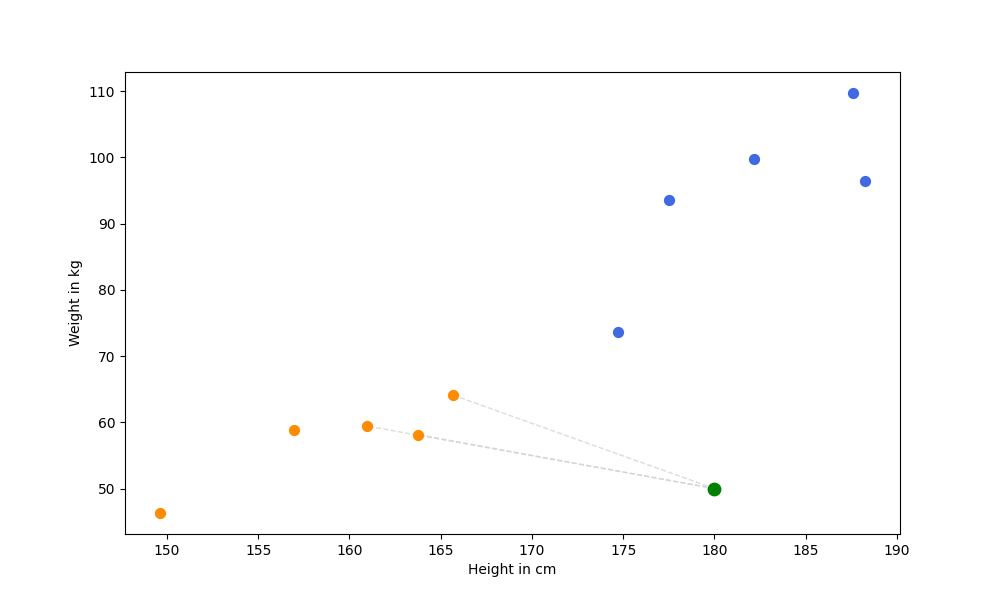
\includegraphics[width=1\linewidth]{Images/kNN/k-NN.png}
    \caption{grapfical depiction of k-NN algorithm}
    \label{fig:my_example}
\end{figure}

\textcolor{red}{\citep{yang2023outlier} for further information}


%After applying the global k-NN, the outlier scores are visualized by the bubble-size
%of the corresponding instance. The color indicates the label, whereas anomalies are red. It can
%be seen, that k-NN cannot detect the anomalies close to the clusters well and assign small
%scores \citep[p.8+9]{goldstein2016comparative}




\subsection*{Minimum Covariance Determinant}
Statistical methods work differently then the methods discussed before. 
The methods making assumptions about the distribution of the data and  estimate population parameters, like mean and covariance.
Resulting in statistical inference, the method can predict with a percentage of how likely it is, that the analysed datapoint is an outlier.
In multivariate dataset, the covariance is an important parameter, because it describes the shape of the data in p-dimensional space.
Therefore using the mahalanobis distance, which incorporates the covariance, can be benefitial.
Naivy, by estimating the mean and covariance matrix and the resulting mahalanobis distance, you could define the $n$ largest distances as ourliers.


But the results of this procedure would be distorted by the masking effect.
Because the sample mean and covariance matrix are themselves sensitive to extreme values, a single outlier can pull the mean toward itself and inflate the covariance, essentially "masking" its own presence and leading to false negatives in outlier detection.
The MCD, proposed in 1984 by \citet{rousseeuw1984least} and later in 1985 theoretically justified in \citet{rousseeuw1985multivariate}, wasproposed as a solution to estimate robust estimators. 
Outliers bias non-robust estimators like the mean, by pullig it towards their direction.


This chapter is organized as follows: First I will explain the goal and the construction of MCD.


\subsection*{Theoretical Foundation}
The goal of MCD is to find a subset $H$ of $h$ \todo{which onw is right? h or n?} observations in a given dataset, with the minimal determinant.
As seen in Fig. the MCD draws the smallest possible ellipsoid, compared to classical methods \todo{which methods?}
When the smallest possible elipsoid is found, a robust distance, like the mahalanobis distance, is used to determine the distances between the subset mean (center) to the specific instance.
Intuitively,  as seen in figure, the goal of MCD is to draw an elipsoid around a subset of the data with the highest local density and not around the complete datatset, which will include outlier. 
Eliminating the masking effect of possible outliers.


%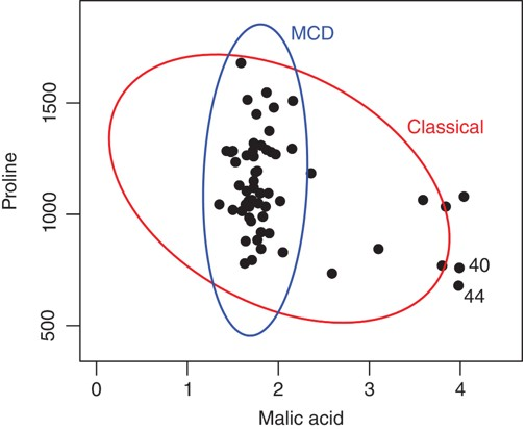
\includegraphics[width=\linewidth]{Images/MCD.pdf}


The MCD has a very high breakdown point.
The breakdown point describes the percentage of abitrary large instances that can be added without the estimator breaks down.
MCD will stay consistens even if 50\% arbirary datapoints are added to the dataset, thats the so called majority rule.
It does this by ignoring the instances outside the subset.
If the abitrary instances get above 50\%, MCD will prioritize those instances and not the subset anymore.
If the outlier ratio does exceed 50\% those cant be named outliers anymore, because they reach the status of inliers, because they are the mayority class. 


MCD is affine equvariant, that means, that the estimators stay consistent if affine transformations are undertaken.
Affine transformations are changes to the data, that does not change the geometric structure of the data.
In data preprocessing are affine transformation often used.
Rescaling data is an affine transformation, but the MCD estimators stay the same, instead of k-NN or deep learning models, that need to be normalized \citet{hubert2018minimum}.
  


\section*{FAST-MCD}
A disadvantage of the original algorithm is that it is computationally complex and for bigger dataset get impossible to estimate.
To find the matrix with the smallest determinant, you have to calculate all possible $\binom{n}{h}$ subsets.  
Therefore a more efficient algorithm, called FAST-MCD, was published in 1999 by \citet{rousseeuw1999fast} which includes concentration steps (C-Steps).
The FAST-MCD estimation is as follows:  

\begin{enumerate}
    \item Determine the number observations $h$ by applying $h = \frac{n+p+1}{2}$
    \item carry out two concentration steps
    \item for the 10 results with lowest $det(S3)$: carry out C-steps until convergence
    \item report the mean and covariance matrix with the lowest $det(S)$
\end{enumerate}
 
Instead it takes many initial choices of Subsets and are applying the concentrantion steps to each until convergence and keept the solution with the lowest determinant.
The C-Step algorithm is as follows:

\begin{enumerate}
    \item Initialize by drawing a random number $p+1$ subsamples $J$ and calculate the sample mean and the sample covariance matrix. If the resulting $det(S0)=0$ then add another random observation until $det(S0)>0$.
    \item If $det(S1)=/0$ compute the mahalanobis distances for all $n$
    \item To compute $H2$ sort the distances of (2) from smallest to biggest
    \item Select the $h$ smallest distances and compute the mean and coverance matrix
    \item Repeat until convergence
\end{enumerate}
\citep[p.214]{rousseeuw1999fast}


\subsection*{Implementation}
As above mentioned, I will calculate just two concentration steps with all initial subsets.
After that I will select the ten results with the smallest determinants.
I will do this selective iteration, because the distinction between robust and nonrobust solutions aleady becomes visible after two or three steps.  
\todo{add:rousseeuw, Driessen (1999)p.216 pp, nested extensions and explain why the algorithm is like this}
If one can be sure, that the dataset contains less then 25\% of outliers, you can choose $h=0.75n$ wich is a good compromise between breakdown value and statistical efficiency.
If the dataset contains many observations (e.g. n > 600), then you can create


\section*{Hyperparameter}
The MCD main hyperparameter is the number of observations in the subset $h$.
The range of $h$ is defined by: 


\begin{equation}
    \frac{n+p+1}{2} \le h \le n. 
\end{equation}


The lower boundary includes a minimum of 50\% of the data and additionaly the number of dimensions $p+1$.
If $p > h$ the resulting determinant of covariance matrix will be 0, hence the covariance matrix can't be inverted and the mahalanobis distances cant be estimated.
\citet{hubert2018minimum} recommends at least five observations per dimension to avaid excessiv noise. 

There is a trade-off relationship between the breakdown value and statistical efficiency.
The higher the robustness is chosen, the less efficient the estimators get. 
If the dataset does not contain more than 25\% of outliers, than it is suitable to choose $h  0.75n$. \citep[p.217]{rousseeuw1999fast}
The newly calculated estimator is less robust, but more efficient then before. 

The resulting $\hat{\mu}_{\text{MCD}}$ is the mean vector of the remaining subset $h$ which is used to calculate the mahalanobis distances.
The Mahalanobis Distance serves as a sophisticated metric for measuring the distance between a data point and the mean of a multidimensional distribution by including the covariance. 
It is defined as follows:


\begin{equation}
    D_M(\mathbf{x}, \mathbf{\mu}) = \sqrt{ (\mathbf{x} - \mathbf{\mu})^T \mathbf{\Sigma}^{-1} (\mathbf{x} - \mathbf{\mu}) }
    \label{eq:mahalanobis}
\end{equation}


Unlike the Euclidean distance, which treats all variables independently, the Mahalanobis Distance accounts for the correlations between dimensions by incorporating the inverse of the covariance matrix. 
This approach effectively standardizes the data, making the metric scale-invariant and allowing it to identify outliers that might appear normal when looking at single variables but are anomalous when viewed in combination.
In a statistical context, if a dataset follows a multivariate normal distribution, the squared Mahalanobis distance follows a Chi-squared distribution. 
This relationship allows researchers to perform parametric tests to flag outliers at a specific significance level. 


To detect outliers, the procedure includes an statisticall hypothesis test \todo{right? discordancy test}.
Testing if the observed datapoint comes from the same multivariante normal distribution as the rest of the data.
To calculate the test statistics, the mahalanobis distance needs to be transformed so it follows a $\chi^2$ distirbution.
The mahalanobis distances is transformed as follows:

\begin{equation}
    RD_i^2 = (\mathbf{x}_i - \hat{\mu}_{\text{MCD}})^T \hat{\Sigma}_{\text{MCD}}^{-1} (\mathbf{x}_i - \hat{\mu}_{\text{MCD}})
    \label{eq:robust_mahalanobis}
\end{equation}

If the mahalanobis distance of the suppodes outlier is greater than the critical $\chi^2$, the probability (p-value) wether this is an inlier is $1- \alpha$.
By increasing $\alpha$, I will increase the size of the elipsoid and an possible outlier has to be further away fromt the $\hat{\mu}_{\text{MCD}}$.
In this case the results will be more certain, but will restrict datapoint to be considered as outliers.


In my thesis I will implement a fixed threshold approach.
To ensure comparability, I will implement approach as described in the other two methods, which is to set the threshold to the outlier ratio.
Therefore, the MCD will rank the distances of datapoints to the MCD mean and the furthest $n\%$ will be defined as outliers.
The hypothesis approach does have an advantage in scenarios, where the outlier ratio is not known.
The detecting is adjusting accourdingly to the unknown outlier ratio.
Nevertheless, the outlier ratio in my experiments is known 


\section*{Variants of MCD}
Even recently reaseach has een done for new extension for MCD.
Because FAST-MCD begins by drawing random subsets, multiple runs of FastMCD on the same dataset may yield different results (a problem often mitigated by fixing the random seed in implementations). 
Furthermore, it requires drawing many initial subsets to ensure at least one is free of outliers, which can be computationally intensive. 
To circumvent both of these problems, the Deterministic MCD (DetMCD) algorithm was developed. \citep[p.621 pp.]{hubert2012deterministic}
DetMCD provides a deterministic approach to robust location and scatter. 
It uses the same iterative steps as FastMCD but avoids starting with random subsets, ensuring consistency. 
Unlike its predecessor, DetMCD is permutation invariant, meaning its result is independent of the order of observations in the dataset. 
Moreover, DetMCD typically runs even faster than FastMCD and is less sensitive to data contamination (outliers).


Briefly, MCD is defined by it high breakdownpoint, which ensures with even a very high outlier ratio a consistent estimation.
MCD does not need normalizations because it is adffine equivariant. 
This eleminates problems with normalization and ensures reliability even if scales are changed.
MCD mitigates the masking problem, making it a supplementary to the statistical hypothesis testing.
Lastly, the statistical approach of MCD making the results transparent and quantifiable, by assigning a probability to every datapoint.


On the opposite, even FAST-MCD is computationally complex and limited by the site of the dataset making it not suitable for modern big data applications.
MCD assumes a gaussian normal distribution and looses performance in dataset with different distributions.
MCD suffers from the Curse of Dimensionality, because it requires more instances than variables. 
The estimation is impossible if this requirement is not met.
FAST-MCD in peticular is a stochastic approach, which means, that two runs can estimate different results.
For solving this problem, there a variance of MCD that to solve it. \citep[p.5]{smiti2020critical}


I chose MCD as a benchmark because of its simplicity and statistical approach compared to the machine-leanring approach of the other methods.
It provides for the given dataset an answer wether the dataset justifies a complex algorithm like InterCont, or if a traditional statsistical method is enough. 
Moreover the affine equivariant charakteristic of MCD provides a second benchmark.
By comparing it to methods, that are not affine equivariant, I expect draw conclusions about the way InterCont learns the underlying geometry of the data \todo{achtung mit dieser aussage}